%%%%%%%%%%%%%%%%%%%%%%%%%%%%%%%%%%%%%%%%%%%%%%%%%%%%%%%%%%%%%
%% Java Time/Date Formatter
%%%%%%%%%%%%%%%%%%%%%%%%%%%%%%%%%%%%%%%%%%%%%%%%%%%%%%%%%%%%%
\chapter{Aufgabe 1}
\label{sec:aufgabe1}

\subsection*{a)}
Schreiben Sie ein Java-Programm, das in einem String Formatspezifikationen gemäß
\textit{java.util.Formatter}
findet. \newline
Erstellen Sie dazu mit der Syntax von
\textit{java.util.regex.Pattern}
einen regulären Ausdruck für eine solche Formatspezifikation. \newline
Sie brauchen darin nicht zu berücksichtigen, dass bestimmte Angaben innerhalb einer Formatspezifikation
nur bei bestimmten Konversionen erlaubt sind.
Achten Sie aber bei argment\_index, width und precision darauf, ob der Zahlbereich bei 0 oder 1 beginnt. \newline
\newline
Beispieleingaben: \newline
\begin{verbatim}
	xxx %d yyy%n
	xxx%1$d yyy
	%1$-02.3dyyy
	Wochentag: %tA Uhrzeit: %tT
\end{verbatim}
	\newline
Beispielausgaben: \newline
\begin{verbatim}
	TEXT("xxx ")FORMAT("%d")TEXT(" yyy")FORMAT("%n")
	TEXT("xxx")FORMAT("%1%d")TEXT(" yyy")
	FORMAT("%1$-02.3d")TEXT("yyy")
	TEXT("Wochentag:")FORMAT("%tA")TEXT("Uhrzeit:")FORMAT("%tT")
\end{verbatim}

\newline

\newpage
\subsection*{a - Lösung}


\subsubsection{Code}
\begin{code}[language=java, caption={Funktion für Java Formatter}, label={lst:Aufgabe1a}]
private static String formatter(String input) {
    Pattern patternGeneral =
            Pattern.compile(
                    "(%([1-9]+\\$)?[-+#0,(\s]?\\d*(\\.\\d)?[bBhHsScCdoxXeEfgGaA%n])"
            );
    Pattern patternDate =
            Pattern.compile(
                    "(%([1-9]+\\$)?[-+#0,(\s]?\\d*[tT][HIklLMSpQZzsBbhAaCYyjmdeRTrDFc])"
            );
    Pattern patternLeftover =
            Pattern.compile(
                    "(%([1-9]+\\$)?[-+#0,(\s]?\\d*\\D)"
            );
    Pattern usePattern = Pattern.compile(
            patternGeneral.pattern()
                    + "|" + patternDate.pattern()
                    + "|" + patternLeftover.pattern()
    );

    var builder = new StringBuilder();

    Map<String, String> parts = new TreeMap<>(Comparator.comparing(input::indexOf));

    Arrays.stream(input.split(usePattern.toString()))
            .forEach(x -> parts.put(x, "TEXT(\"" + x + "\")"));

    usePattern.matcher(input).results()
            .forEach(x -> parts.put(x.group(), "FORMAT(\"" + x.group() + "\")"));

    parts.forEach((x, y) -> builder.append(y));

    return builder.toString();
}
\end{code}

\subsubsection{Erklärung}
Das Pattern ist realisiert anhand der \href{https://docs.oracle.com/javase/7/docs/api/java/util/Formatter.html}{Java Formatter Docs}. \newline

Dazu unterteilen wir in 3 Unterscheidungen:
\begin{itemize}
	\item generelle Formate
  \item Datum
  \item Rest/Unspezifiziert
\end{itemize}

Was sich alle Formate teilen, ist das beginnende \verb|'%'|.
Formate erlauben einen optionalen Format-Index anzugeben: \verb|'([1-9]+\$)?'|, sowie verschiedene Formattierungs-Optionen: \verb|'[-+#0,( ]?'| und eine optionale Angabe für die
minimale Anzahl an Charakteren: \verb|'\d*'|.\newline
Zusammengehängt ergibt das: \verb|'%([1-9]+\\$)?[-+#0,(\s]?\\d*'|.

Bei den generellen Formaten gibt es die zusätzliche Option für die Anzahl Nachkommastellen: \verb|'(\.\d)?'| gefolgt von den möglichen Konversionen: \verb|'[bBhHsScCdoxXeEfgGaA%n]'|.\newline
Für ein Datum fehlt noch \verb|'[tT]'| und Konversionen: \verb|'[HIklLMSpQZzsBbhAaCYyjmdeRTrDFc]'|.\newline
Alle restlichen Konversionen sind illegal und reserviert für zukünftige Erweiterungen. Diese decken wir mit \verb|'\D'| ab.

Anschließend wird der String in einzelne Teile zerlegt, die dann in einer Map gespeichert werden.
Sortiert wird anhand der Position des Keys im Input-String. \newline
Die fertige Map wird dann in einen String umgewandelt. \newline

\subsubsection{Programmausgabe}

\begin{code}[language=java, caption={Input für Formatter}, label={lst:Aufgabe1a_in}]
public static void main(String[] args) {
  System.out.println(formatter("xxx %d yyy%n"));
  System.out.println(formatter("xxx%1$d yyy"));
  System.out.println(formatter("%1$-02.3dyyy"));
  System.out.println(formatter("Wochentag: %tA Uhrzeit: %tT"));
}
\end{code}

\begin{figure}[h]
	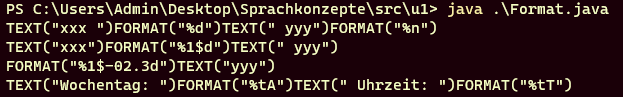
\includegraphics[width=\textwidth]{media/Aufgabe1a_formatter_output}
	\caption{Ausgabe Java Formatter}
	\label{img:Aufgabe1a_output}
\end{figure}

\newpage

\subsection*{b)}
Erkennen Sie mit ANTLR 4 Lexer-Regeln Zeitangaben im digitalen 12-Sunden-Format gemäß \url{https://en.wikipedia.org/wiki/12-hour_clock}.
Beachten Sie auch die alternativen Schreibweisen 12 midnight und 12 noon. Testen Sie mit \textit{org.antlr.v4.gui.TestRig}.

\subsection*{b - Lösung}

\subsubsection{Code}
\begin{code}[language=antlr, caption={Lexer für Date/Time}, label={lst:Aufgabe1b}]
    lexer grammar TimeLexer;

    Time12H: Default|Noon|Midnight;

    fragment Default: ('12:00'|(([1-9]|'1'[01])':'[0-5][0-9]))WS[ap]'.m.';
    fragment Noon: 'Noon'|'12 noon';
    fragment Midnight: 'Midnight'|'12 midnight';

    WS: [ \t\r\n]+ -> skip;
\end{code}

\subsubsection{Erklärung}
\textbf{Lexer Grammatiken beschreiben die Token, die vom Lexer erkannt werden sollen.}
Fragmente sind Teile der Grammatik, die nicht direkt erkannt werden, sondern nur in anderen Regeln verwendet werden. \newline
Der Ansatz hier war die Zeitangaben in drei Teile zu zerlegen: \newline
\begin{itemize}
    \item Default: Volle Uhrzeitangaben im klassischen `HH:MM' Format mit AM/PM Angabe
    \item Noon: Zusätzlich die Mittagszeit `12 noon' und `Noon'
    \item Midnight: Synchron dazu Mitternacht `12 midnight' und `Midnight'
\end{itemize}
Noon und Midnight sind hierbei die Ausnahme, aber vorgegeben durch die Aufgabenstellung. \newline

\newpage

Alternativ könnte man mehr Token beschreiben:
\begin{code}[language=antlr, caption={alternativer Lexer}, label={lst:Aufgabe1bV2}]
    lexer grammar TimeLexerV2;

    TIME : HOUR SEPERATOR MINUTE (AM | PM)
    | TWELVE SEPERATOR '00' (AM | PM)
    | TWELVE 'noon'
    | TWELVE 'midnight'
    | 'Noon'
    | 'Midnight';

    TWELVE : '12';

    HOUR : '1'[0-1]|[0-9];
    MINUTE : [0-5][0-9];
    SEPERATOR : ':';

    AM : 'a.m.' ;
    PM : 'p.m.' ;

    WS: [ \t\r\n]+ -> skip;
\end{code}
Allerdings wird die Lexer Grammatik hier etwas missbraucht, da die `TIME' Regel eher als Parser Regel genutzt wird.
Lexer Regeln sollten eigentlich nur die Token beschreiben, die vom Lexer erkannt werden sollen. \newline


\subsubsection{Programmausgabe}

Korrekter Input:
\begin{verbatim}
12:00 AM
12:00 a.m.
12:00 am
3:00 am
1:12 am

Noon
12 noon
Midnight
11:59 PM
\end{verbatim}

\begin{figure}[H]
	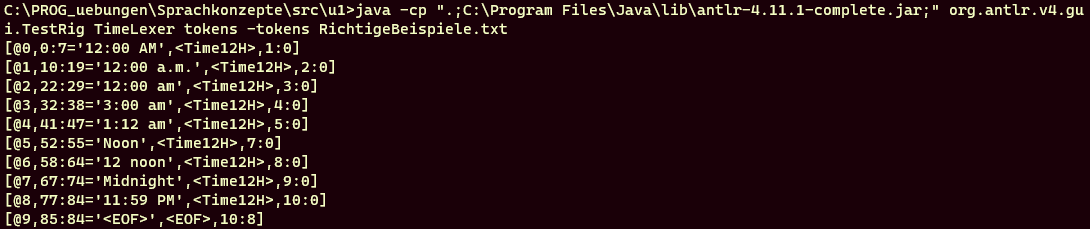
\includegraphics[width=\textwidth]{media/Aufgabe1b_correct_test}
	\caption{Ausgabe TimeLexer richtiger Input}
	\label{img:Aufgabe1b_correct_test}
\end{figure}

Falscher Input:
\begin{verbatim}
0:00 am
0:00 pm
12:00
noon
12 Noon
13:00 PM
\end{verbatim}

\begin{figure}[H]
	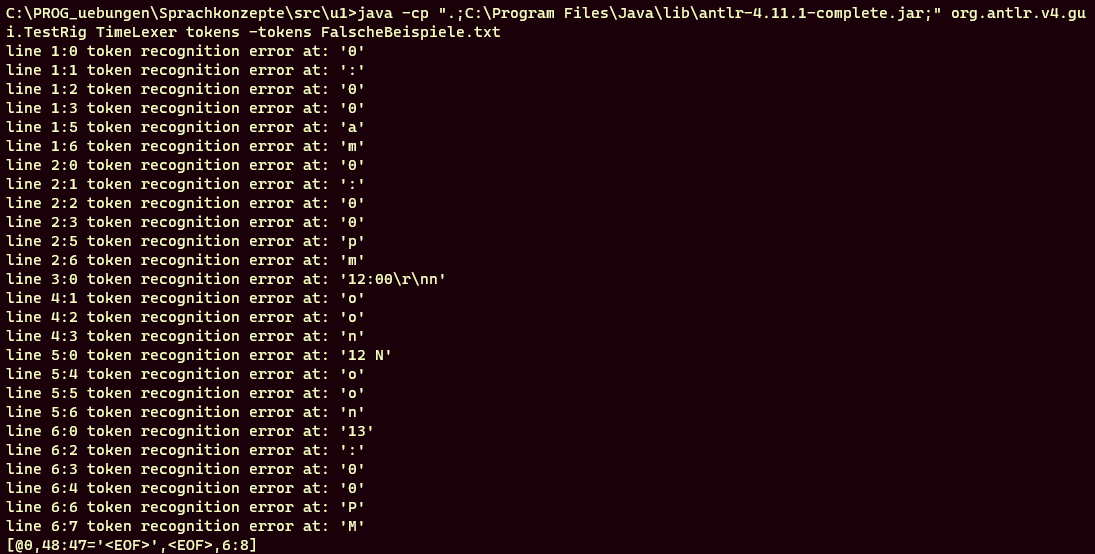
\includegraphics[width=\textwidth]{media/Aufgabe1b_wrong_test}
	\caption{Ausgabe TimeLexer falscher Input}
	\label{img:Aufgabe1b_wrong_test}
\end{figure}


\newpage